\documentclass{beamer}
\usepackage[utf8]{inputenc}
\usepackage{amsmath}
\usepackage{amsfonts}
\usepackage{amssymb}
\usepackage{algorithm}
\usepackage{algpseudocode}

\usetheme{metropolis}

\makeatletter
\algrenewcommand\ALG@beginalgorithmic{\footnotesize}
\makeatother

%Information to be included in the title page:
\title{Scheduling on an Asymmetric Multicore System}
\author{Ren Wall, Nic Rust, Gavin Austin}
\institute{}
\date{12 Dec 2019}

\begin{document}
	\frame{\titlepage}
	
	\begin{frame}
		\frametitle{Asymmetric Multicore systems.}
		ARM big.LITTLE systems\\
		Large X86-64 CPUs with different speed cores.\\
		\includegraphics[width=7cm]{images/ARMCortexA57A53.jpg}
	\end{frame}
	
	\begin{frame}
		\frametitle{Optimization Goals \cite{AAP2013}}
		Computation time\\
		Power Consumption\\
		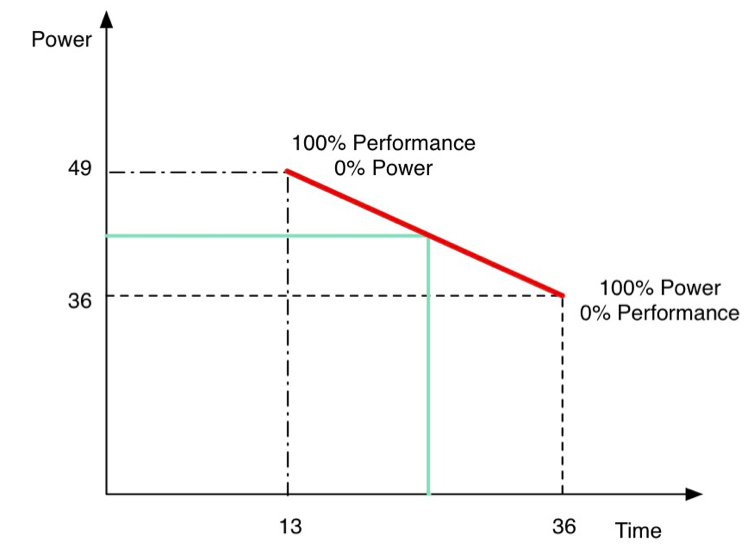
\includegraphics[width=7cm]{images/power_vs_performance.jpg}
	\end{frame}
	
	\begin{frame}
		\frametitle{Energy Aware Scheduler (EAS)\cite{EAS2015}}
		EAS is the first Linux implementation of the CFS with built in idling and frequency tuning.\\
		Implemented in 2015.\\
		Greatly improves upon previous iteration.\\
		\cite{EASp2015}
	\end{frame}
	
	\begin{frame}
		\frametitle{Improvements Over Previous Scheduler\cite{EASp2015}}
		cpuidle vs sched-idle\\
		cpufreq vs sched-freq\\
	\end{frame}
	
	\begin{frame}
		\frametitle{Drawbacks of EAS}
		If all cores are at full capacity its just a CFS.
	\end{frame}
	
	\begin{frame}
		\frametitle{WASH Compared to EAS}
		Wash always schedules on highest power core.\\
		Thread priorities arranged by most contended held locks.\\
		Most waited on thread is placed on fastest core.\\
		\begin{figure}[h]
			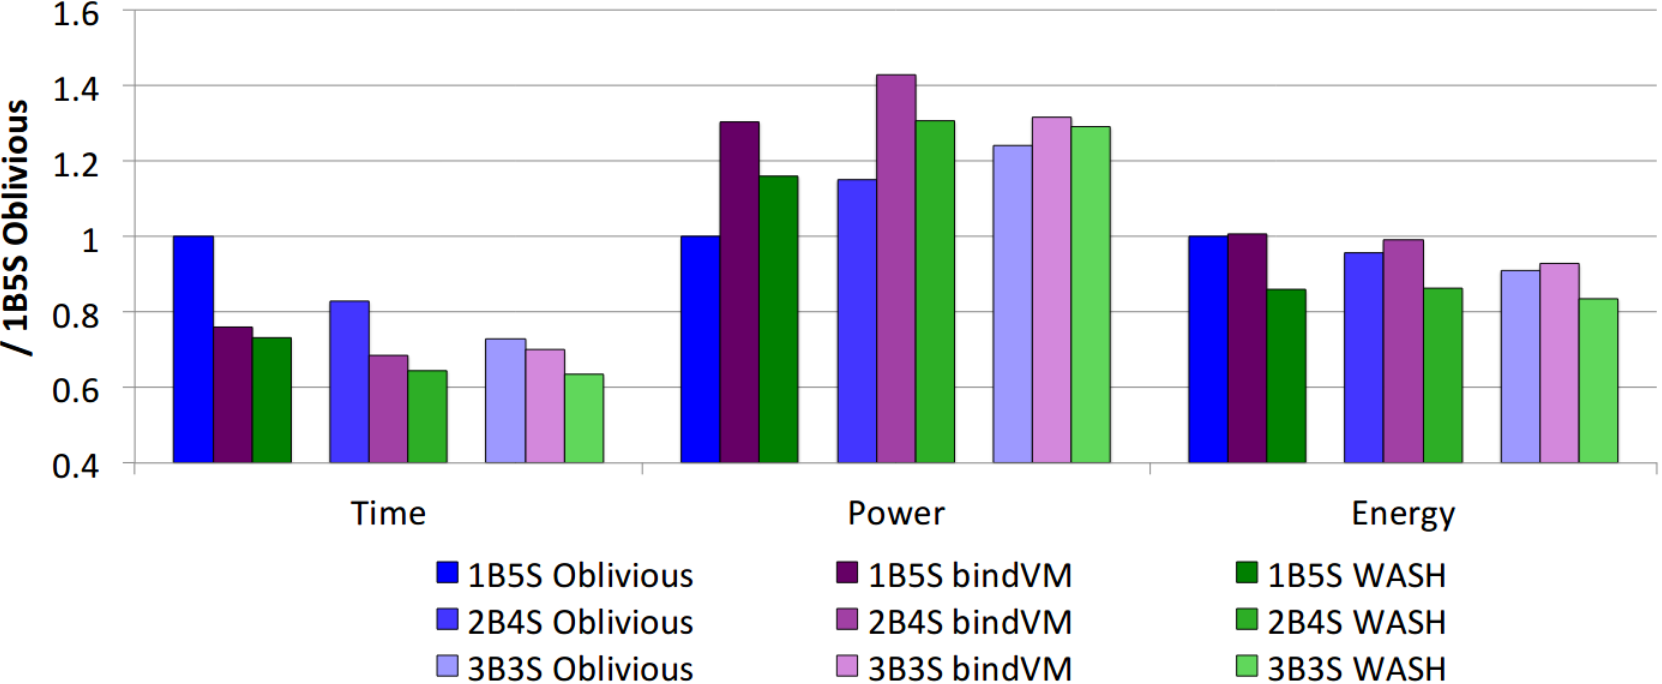
\includegraphics[width=\textwidth]{images/WASH_benchmarks.jpg}
			\caption{CFS (Oblivious), manual core prio (bindVM); 1B5S (1Big core and 5 Small cores), 2B4S and 3B3S \cite{Jibaja:2016:PPA:2854038.2854047}.}
			\label{fig:WASH_benchmarks}
		\end{figure}
	\end{frame}
	
	\begin{frame}
		\frametitle{WASH Scheduler}
		\vspace*{-2.5mm}
		\begin{algorithm}[H]
		\caption{WASH}\label{euclid}
		\begin{algorithmic}
			\Function{WASH}{$T_A,T_V,C_B,C_S,t$}
				\State $T_A$: Set of application threads
				\State $T_V$: Set of VM service threads, $T_A \cap T_V = \emptyset$
				\State $C_B$: Set of big cores
				\State $C_S$: Set of small cores, $C_B \cap C_S = \emptyset$
				\State $t$: Thread to schedule where $t \in T_A \cup T_V$
				\If{$|T_A| \leq |C_B|$}
					\If{$t \in T_A$}{ Set Affinity of t to $C_B$ }
					\Else{ Set Affinity of $t$ to $C_B \cup C_S$}
					\EndIf
				\ElsIf{$t \in T_A$}
					\If{$\forall \tau \in T_A (\text{Lock\%}(\tau) \le \text{Lock}_{\text{Thresh}})$}
						\State Set Affinity of $t$ to $C_B \cup C_S$
					\EndIf
				\EndIf
			\EndFunction
		\end{algorithmic}
		\end{algorithm}
		\vspace*{-7mm}
		Psudocode from \cite{Jibaja:2016:PPA:2854038.2854047}
	\end{frame}
	
	\begin{frame}
		\bibliographystyle{amsalpha}
		\bibliography{bibliography}{}
	\end{frame}
\end{document}